\section{Tracking System}

\subsection{Introduction}

To accurately simulate a volumetric display, it is essential to determine the positions of the user's face and hands, which allows for rendering the correct perspective for the user. To achieve this, our tracking system needed to meet the following requirements:

\begin{itemize}[itemsep=-0.25em]
	\item \textbf{High resolution:} Precisely track the user's eyes and hands.
	\item \textbf{High framerate:} Ensure smooth tracking of the user's eyes and hands.
	\item \textbf{Low latency:} Provide near real-time tracking of the user's face and hands.
\end{itemize}
%%%%%%%%%%%%%%%%%%%%%%%%%%%%%%%%%%%%%%%%%%%%%%%%%%%%%%%%%%%%%%%%%%%%%%%%%%%%%%%%%%%%%%%%%%%%

\subsection{Hardware}

\begin{figureBox}[label={fig:kinect}, width=0.4\linewidth]{Azure Kinect \cite{noauthor_buy_nodate}}
    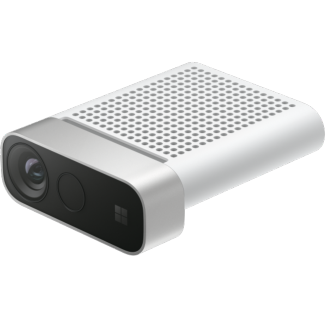
\includegraphics[width=0.9\linewidth]{./implementation/figures/kinect.pdf}
\end{figureBox}

For this project, we used a Microsoft Azure Kinect camera (Fig~\ref{fig:kinect}). The Azure Kinect camera is equipped with two sensors: a depth sensor (utilizing an IR camera) and a color camera. \\

We configured the camera to capture images at its widest field of view (FoV) of $90^{\circ} \times 74.3^{\circ}$, with an exposure time of 12.8 ms and a framerate of 30 fps. To use this configuration, we compromised on the resolution of the color images, running the RGB camera at $2048 \times 1536$ instead of its maximum resolution of $4096 \times 3072$. Similarly, we used the depth camera at a $2\times2$ binned resolution of $512 \times 512$, instead of its maximum unbinned resolution of $1024 \times 1024$. \\

Because we utilized the depth camera in wide FoV mode ($120^{\circ} \times 120^{\circ}$), rather than the narrower FoV mode ($75^{\circ} \times 65^{\circ}$), the maximum operating range of the depth sensor was reduced to 2.88 m, compared to 5.46 m in the narrower FoV mode. This reduction in range was acceptable for our purposes, as the user was expected to be within 1.5 m of the camera.

%%%%%%%%%%%%%%%%%%%%%%%%%%%%%%%%%%%%%%%%%%%%%%%%%%%%%%%%%%%%%%%%%%%%%%%%%%%%%%%%%%%%%%%%%%%%

\subsection{Core Libaries}  

\subsubsection{Azure Kinect SDK (K4A)}

We utilize the Azure Kinect SDK (K4A) \cite{noauthor_microsoftazure-kinect-sensor-sdk_2024} library to retrieve captures from the Kinect and handle the spatial transformations necessary to calculate the positions of points in 3D. \\

When the Kinect camera is polled using the K4A library, it returns a "Capture," which is a struct containing a color image, a depth image, and an IR image. It is important to note that the depth image is in a different coordinate space compared to the color image, as illustrated in Fig~\ref{fig:diff-spaces}. This discrepancy arises because the color image and depth/IR image are captured using physically offset sensors, resulting in a slight variation in perspective. The depth image resides in what is known as "depth space," while the color image resides in "color space." To utilize these two images together, they must be converted to the same coordinate space. \\

\begin{figureBox}[label={fig:diff-spaces}, width=0.8\linewidth]{Different Spaces: Depth and Color Images \cite{noauthor_use_nodate}}
    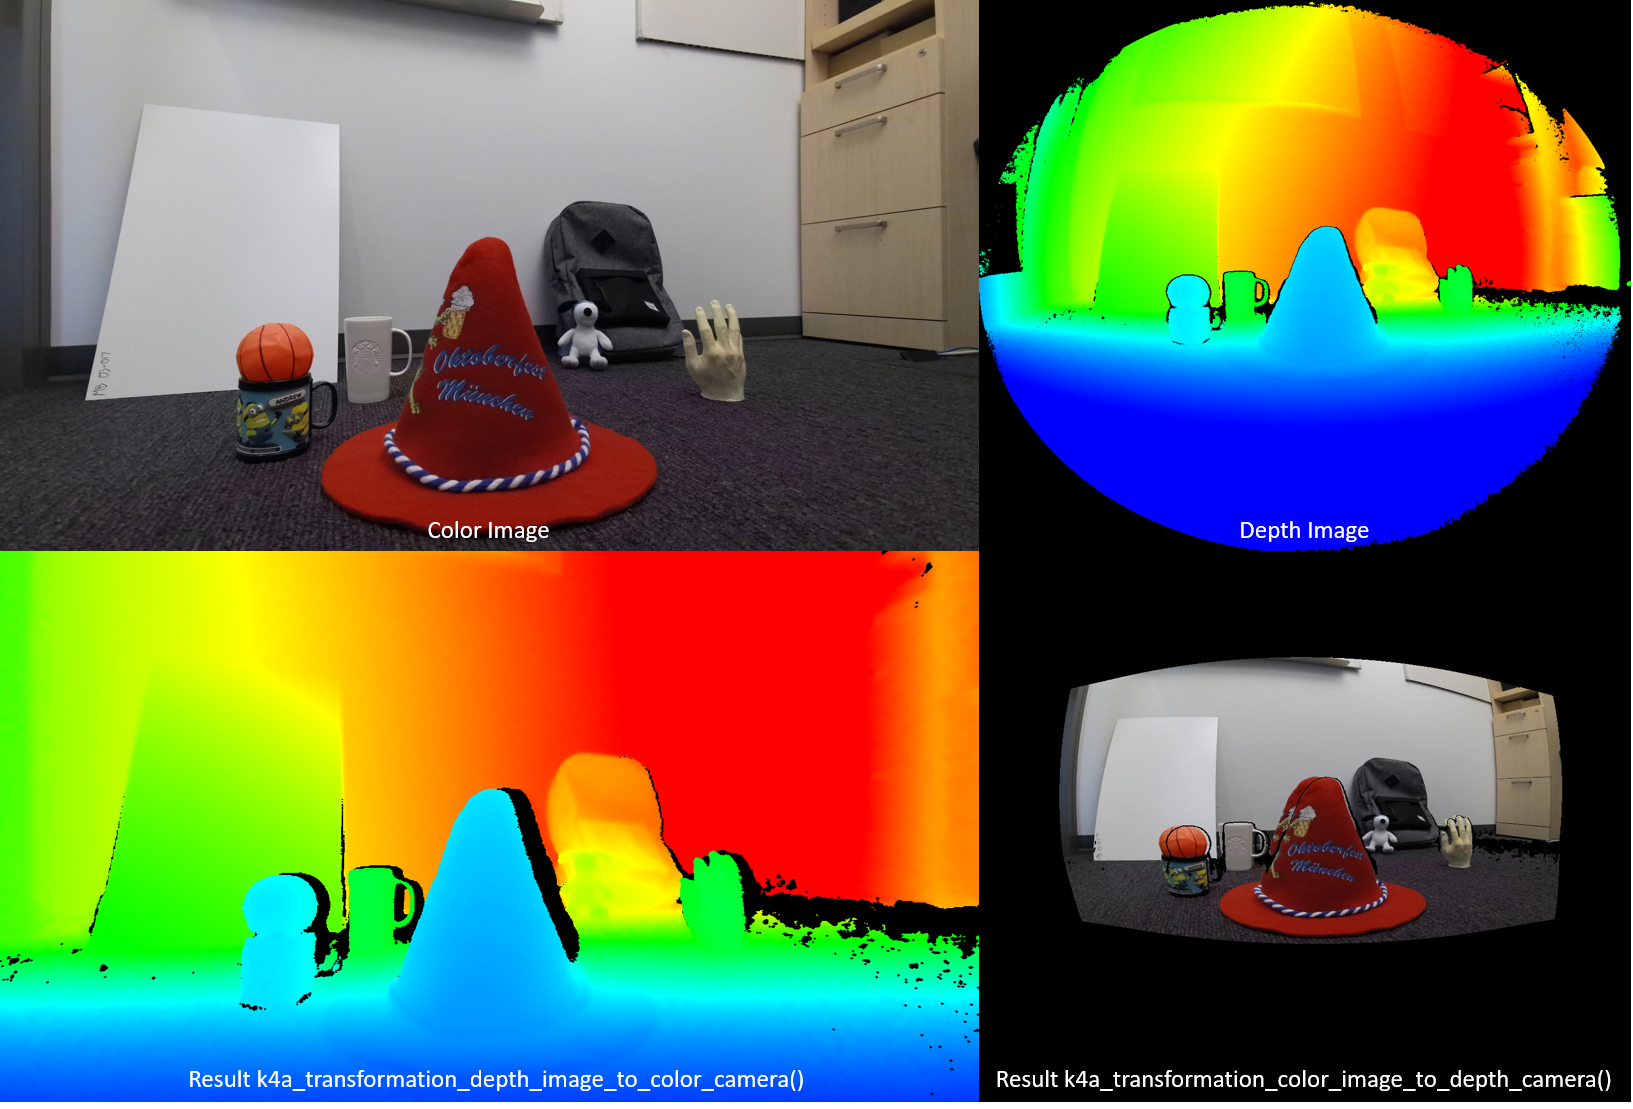
\includegraphics[width=1.0\linewidth]{./implementation/figures/different spaces.png}
\end{figureBox}

Using a "calibration" that is generated at the start of the program, K4A allows conversion between the four different "spaces": "Depth 2D," "Depth 3D," "Color 2D," and "Color 3D." There are notable performance implications when using different spaces for various tasks. For instance, converting from "Depth 2D" to "Depth 3D" is significantly faster than converting from "Color 2D" to "Color 3D." \\

An interesting side effect of converting between spaces is that, due to the physical offset and different diffraction characteristics of the IR and color cameras, "depth shadows" \cite{Kersten1997-so} can occur, as visible in the bottom left image in Fig~\ref{fig:diff-spaces}. These depth shadows can complicate tracking thin objects, such as fingers, because they increase the likelihood of encountering invalid depth data. We explored using the IR image for tracking to mitigate these depth shadows; however, we found that tracking models struggled with IR images, leading us to continue using the original color image method.

\subsubsection{OpenCV}

We use OpenCV \cite{bradski2008learning} to handle the images obtained from the Azure Kinect SDK. OpenCV is a comprehensive library that provides a wide range of functions for image processing and computer vision. We utilize OpenCV to convert the images from the Azure Kinect SDK into a format that can be efficiently processed by Dlib and MediaPipe. We leverage OpenCV's GPU/CUDA-accelerated functionalities, such as image pyramids for downscaling, to enhance the performance of our tracking system. Additionally, OpenCV is used for debugging purposes to render images to the screen.

\subsubsection{Dlib}

We use Dlib \cite{dlib09} for tracking the user's face. Dlib is a modern C++ toolkit that includes machine learning algorithms and tools for creating complex software solutions in C++. As discussed in greater detail later in this section, we use Dlib's face tracking model to track the user's eyes. We also utilize Dlib's GPU-accelerated functions to improve the performance of our tracking system.

\subsubsection{MediaPipe}

We use MediaPipe \cite{lugaresi2019mediapipe} for tracking the user's hands. MediaPipe is a cross-platform framework designed for building multimodal applied machine learning pipelines. We employ MediaPipe's hand tracking model on color images to track the user's hands in real-time. MediaPipe's hand tracking model is a deep learning model capable of accurately tracking hand movements in real-time.


%%%%%%%%%%%%%%%%%%%%%%%%%%%%%%%%%%%%%%%%%%%%%%%%%%%%%%%%%%%%%%%%%%%%%%%%%%%%%%%%%%%%%%%%%%%%

\subsection{Overall Tracking System Design}

The primary goal of the tracking system is to convert the captures provided by the Kinect camera into 3D points that represent positional information, such as the positions of the user's eyes and fingers. The current system focuses on returning the position of the left eye and the tips of the index and middle fingers on the hand closest to the camera. The system operates smoothly at the same frame rate as the Kinect camera, which is 30 frames per second (fps). \\

Several different approaches were considered for the tracking system design. Ultimately, we chose to use a method that tracks the positions of the user's face and hands separately using 2D color images. These images are then processed and converted into 3D points. \\

An alternative approach we considered was to track the face and hands directly in 3D. However, we decided against this method for several reasons. Although the rendering system is an important aspect of this project, it was not our primary focus, and we were concerned that tackling 3D tracking would be too complex given our time constraints. The ecosystem for 2D tracking is more mature, partly due to advancements driven by mobile phone technology, allowing us to leverage existing work, such as the Dlib, MediaPipe, and OpenCV libraries discussed previously. Additionally, we were concerned about the performance of 3D tracking. The increased data volume associated with 3D tracking could potentially slow down the system, making it difficult to achieve real-time tracking of the user's face and hands. \\

Despite opting for 2D tracking, there are several downsides to this approach. For example, as discussed further in the evaluation section, it can be challenging to accurately determine the positions of objects in 3D space that are occluded, such as fingers behind other fingers. Fingers, being relatively small objects, require sampling a general area to identify their position, and selecting the closest valid point. If only the predicted point is sampled, there is a risk of missing the finger and encountering a "depth shadow".

\begin{figureBox}[label={fig:tracker-overview}, width=1.0\linewidth]{Tracker Overview}
    \includegraphics[width=1.0\linewidth]{./implementation/figures/tracker.pdf}
\end{figureBox}

As illustrated in Fig~\ref{fig:tracker-overview}, the process flow of the tracking system is as follows:

\begin{enumerate}[itemsep=-0.25em]
    \item \textbf{Retrieve Capture:} The Kinect Camera is polled to receive a capture.
    \item \textbf{Run Tracking:} Hand and head tracking are performed on the color image.
    \item \textbf{Extract Key Features:} The positions of the tracked points are extracted from the hands (middle and index fingertips) and face (left eye).
    \item \textbf{Convert to 3D:} The depth image is sampled to convert the 2D points into 3D points, which are then placed in a "tracking frame" to be sent to the renderer.
\end{enumerate}

While it might seem unconventional, we maintain separate instances for tracking the left eye and the thumb and index fingertips. This approach is necessary because there is no guarantee that the tracker will detect both the face and hands in a single pass through. For instance, if the user holds their hand in front of their face, the tracker may only detect the hand. Additionally, there is a possibility that either of the tracking models may fail to detect the intended features. In such cases, our system will reuse the last known position and the corresponding capture, which serves as a reasonable approximation for the eye or finger positions. This strategy also helps to reduce the jerkiness effect that can occur with sporadic dropouts. \\

It is important to note that, for performance reasons, we do not calculate the 3D positioning of the points until the renderer requests them. This approach minimizes resource wastage. If we can process a capture faster than the renderer can render a frame, we only calculate the 3D positioning for the most recent capture.

\subsection{Tracking Models}

\subsubsection{Dlib}
We use Dlib to track the left eye's position through a two-stage process. In the first stage, we utilize a Max-Margin Object Detection model \cite{king2015maxmargin, noauthor_dlib_nodate} implemented with a convolutional neural network (CNN) \cite{DBLP:journals/corr/Schmidhuber14}. Instead of training our own model, we used a pre-trained model provided by Dlib \cite{noauthor_index_nodate}, known as \texttt{mmod\_human\_face\_detector}. Initially, we ran the face detection model on the CPU; however, this created a bottleneck in our tracking pipeline. Therefore, we opted to run our CNN on a GPU using CUDA-accelerated functions to meet our performance requirements. \\

Once the user's face is detected, we proceed to the second stage of our facial landmark detection model. We chose to use a five-landmark pose estimator called \texttt{shape\_predictor\_5\_face\_landmark}, leveraging Dlib's implementation of a method proposed in "One Millisecond Face Alignment with an Ensemble of Regression Trees" \cite{6909637}, trained on the iBUG 300-W face landmark dataset \cite{6755925}. This pose estimator operates efficiently enough on a CPU, so GPU acceleration was unnecessary. \\

An example of the results obtained from running the two Dlib models can be seen in Fig~\ref{fig:face-tracker}.

\begin{invisBox}
    \pictureBox[label={fig:face-tracker}]{Dlib Face Tracker}{
        \adjustbox{height=5.75cm, keepaspectratio}{
            \includegraphics{./implementation/figures/Face-tracker.png}
        }
    }
    \hfill
    \pictureBox[label={fig:hand-tracker}]{MediaPipe Hand Tracker}{
        \adjustbox{height=5.75cm, keepaspectratio}{
            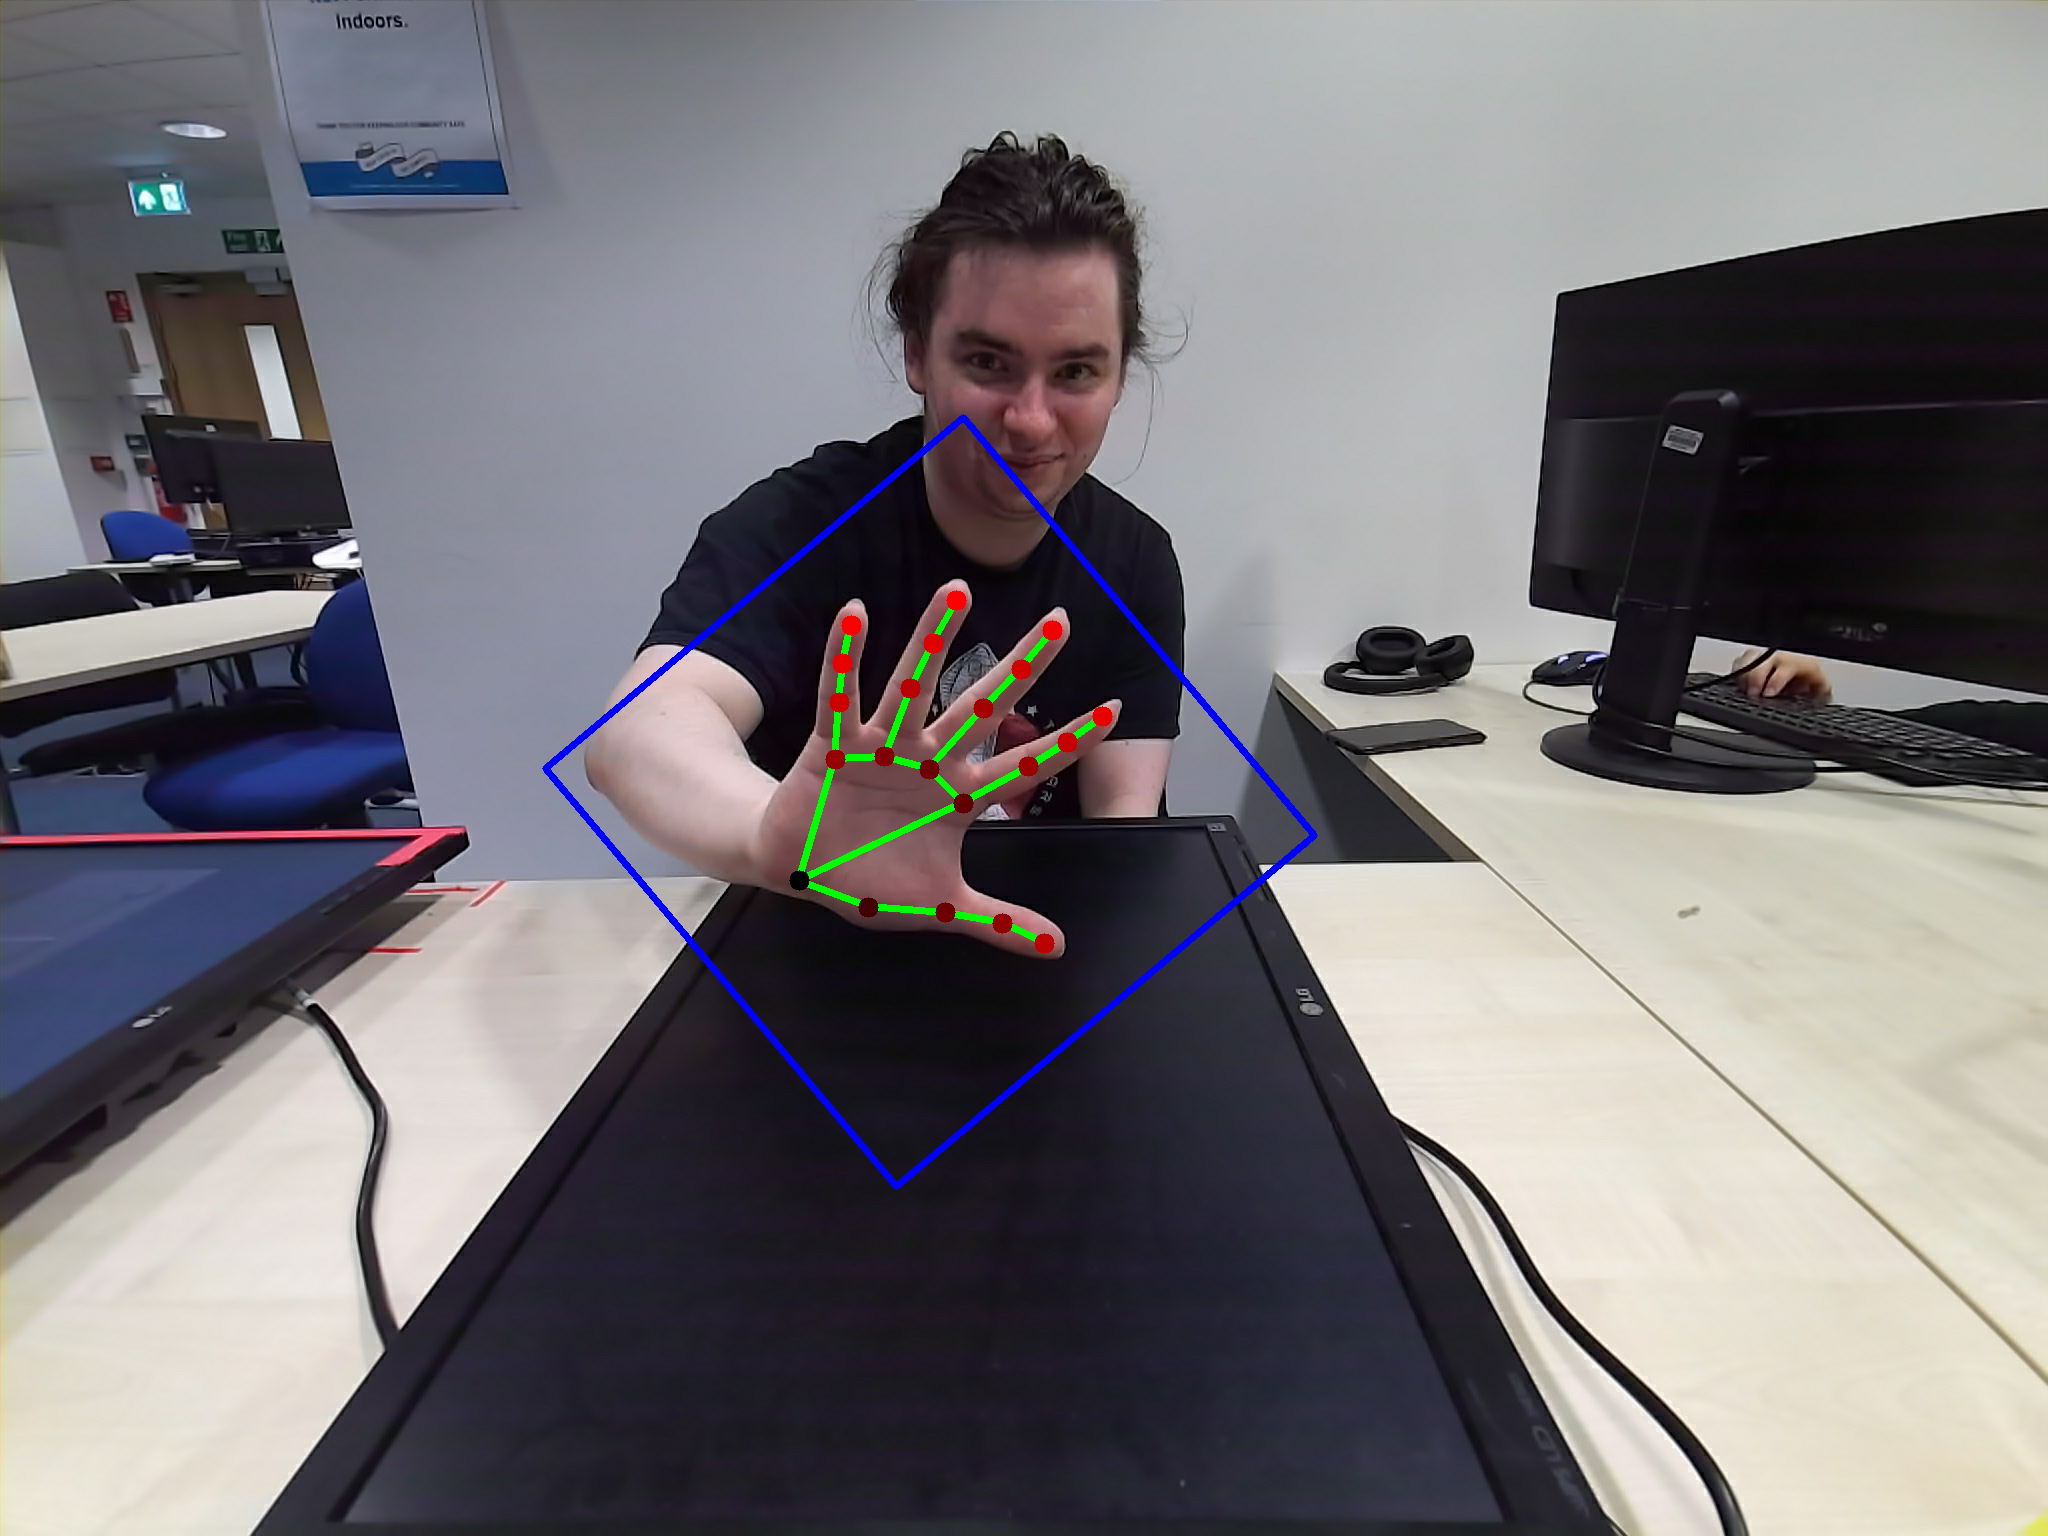
\includegraphics{./implementation/figures/hand-tracker.png}
        }
    }
\end{invisBox}

\subsubsection{MediaPipe}
We use MediaPipe to track the position of two fingers on the user's hand, employing a two-stage process. MediaPipe uses a two-stage model to track hands \cite{zhang2020mediapipe}. The first stage involves a palm detection model that identifies the position of the hand within the image. The second stage is a hand landmark model that detects the positions of 21 points on the hand. MediaPipe provides an interface that allows us to feed images as a stream, abstracting away most of the detection logic, unlike Dlib. \\

We chose to track the positions of the index and middle fingers because this configuration proved to be more stable than tracking the thumb and index finger, and it led to fewer instances of accidental occlusion. To enhance the tracking accuracy, we depth-sample from the surface of the hand and apply a constant offset to make it appear as though the point is inside the hand. An example of the results from running the two MediaPipe models can be seen in Fig~\ref{fig:hand-tracker}.

\subsubsection*{Downscaling}
To ensure that our tracking system operates at a sufficient frame rate, we downscale the images obtained from the camera. We found that downscaling the images using an image pyramid \cite{adelson1984pmi} by a factor of 2 still yields accurate tracking results. This significantly improves the performance of our tracking system. Further details can be found in the evaluation section.

%%%%%%%%%%%%%%%%%%%%%%%%%%%%%%%%%%%%%%%%%%%%%%%%%%%%%%%%%%%%%%%%%%%%%%%%%%%%%%%%%%%%%%%%%%%%

\subsection{Multithreading}

One of the more challenging aspects of this project was making our tracking system performant enough to feel smooth and responsive. To achieve this, we implemented a multi-threaded design, as outlined in Fig~\ref{fig:mult-threaded-des}. We used separate threads for tracking, capturing, and rendering.

\begin{figureBox}[label={fig:mult-threaded-des}, width=0.8\linewidth]{Multi-threaded Design}
    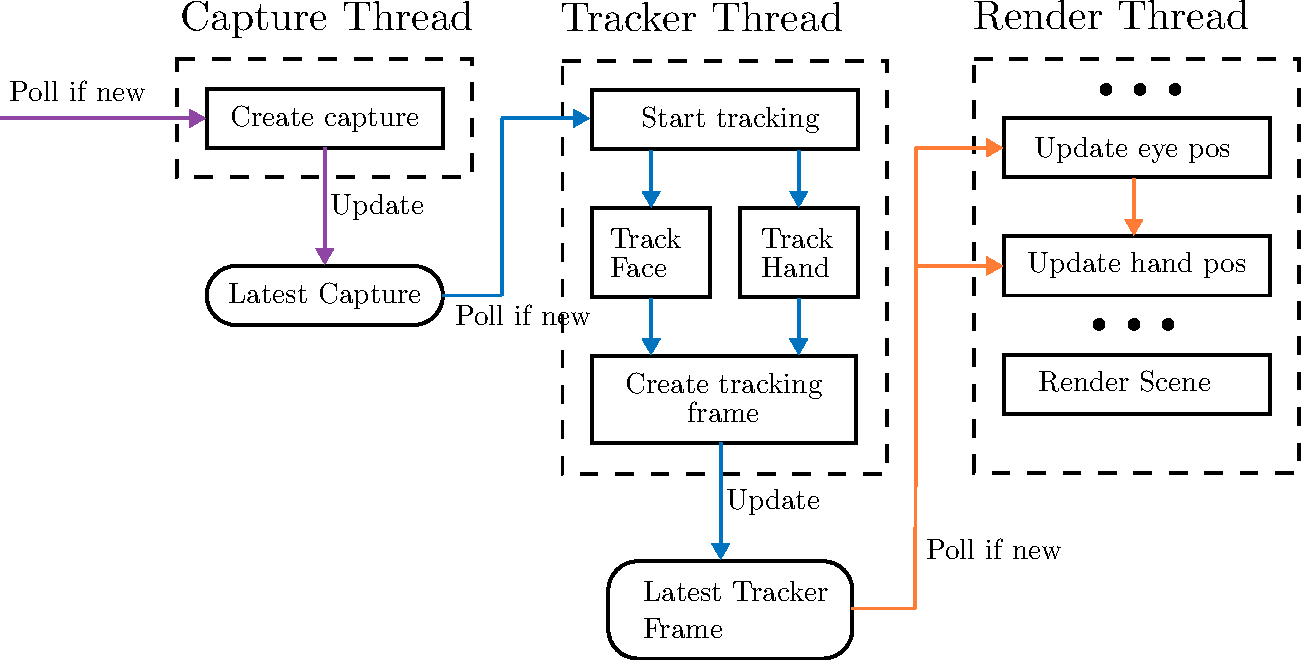
\includegraphics[width=1.0\linewidth]{./implementation/figures/multi-thread-design.pdf}
\end{figureBox}

The purpose of this design was to ensure that the tracking thread and models were utilized 100\% of the time, as they are the most computationally intensive components of the system and represent the main bottleneck. While using a multithreaded design does not reduce the system's latency (as discussed further in the evaluation section), it significantly increases the application's throughput and frame rate.

\begin{figureBox}[label={fig:single-vs-multi}, width=0.8\linewidth]{Single vs Multi-threaded Design}
    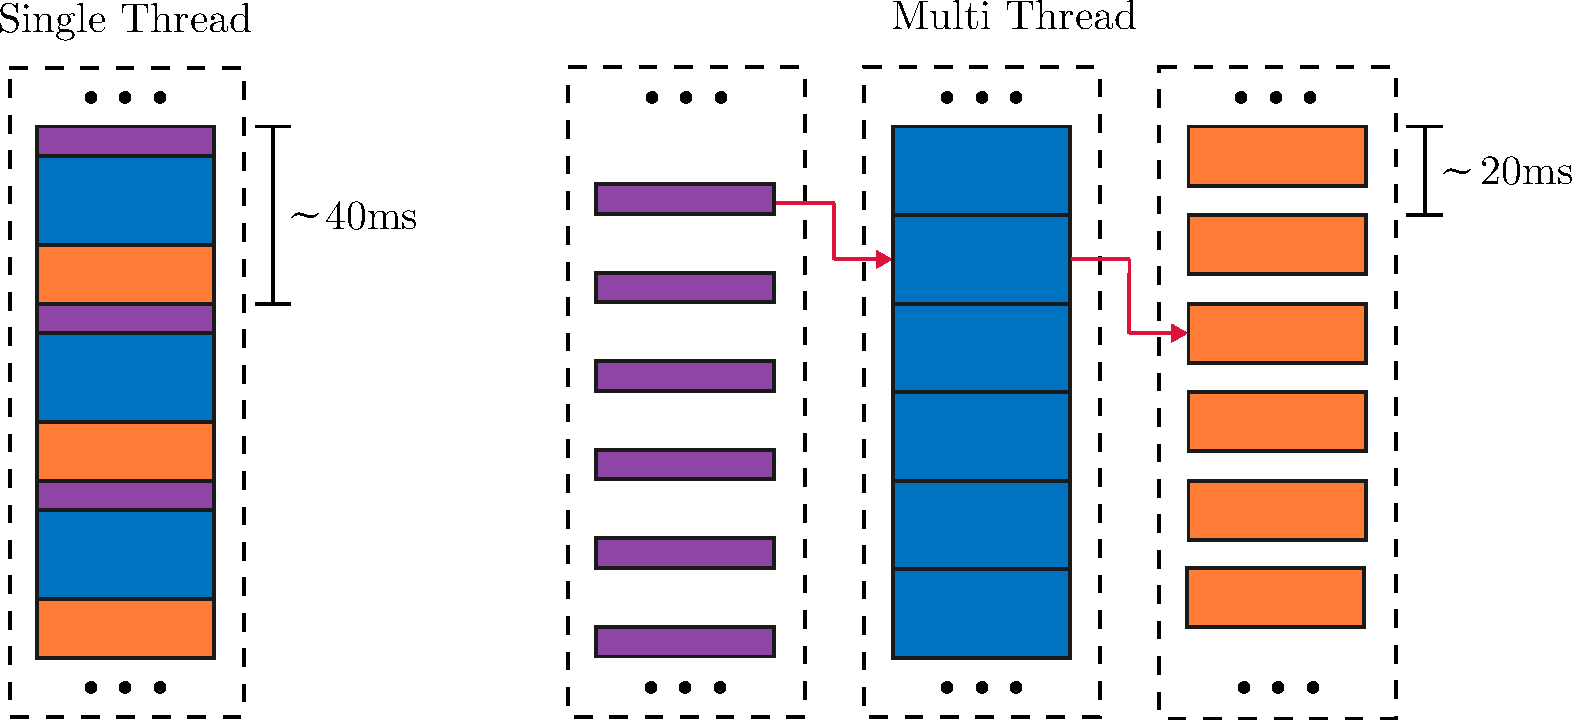
\includegraphics[width=0.8\linewidth]{./implementation/figures/single-vs-multi.pdf}
\end{figureBox}

Since the Kinect camera operates at 30 fps, we need to process an image every $ \frac{1000 \text{ ms}}{30} = 33.3 \text{ ms}$ to ensure that we handle every frame. In our initial single-threaded implementation, we were unable to achieve this rate. By switching to a multi-threaded design, we decreased the time required to produce a new tracking frame to match the duration of the slowest thread (the tracker thread), as shown in Fig~\ref{fig:single-vs-multi}. This also allowed us to run the simulation at a frame rate independent of the tracker. Although this design resulted in the capture thread often being idle, the overall system was light on resources, making this trade-off worthwhile for the significant frame rate improvement it provided.

%%%%%%%%%%%%%%%%%%%%%%%%%%%%%%%%%%%%%%%%%%%%%%%%%%%%%%%%%%%%%%%%%%%%%%%%%%%%%%%%%%%%%%%%%%%%

\subsection{GPU Acceleration}

Another method we utilized to enhance the performance of our tracking system is GPU/CUDA acceleration. Both Dlib and MediaPipe support GPU acceleration. However, we only needed to use GPU acceleration in Dlib because the CPU speed was already sufficient for our tracking pipeline in MediaPipe. The reported speedup of 12.27 ms with GPU acceleration versus 17.12 ms without \cite{noauthor_hand_nodate} did not justify the effort required to enable CUDA in MediaPipe, especially given the complexities involved in building with Nix (see the build systems section for more information). \\

As illustrated in Fig~\ref{fig:system-des}, we only used GPU acceleration for two parts of our tracking system, excluding rendering. We utilized OpenCV's GPU-accelerated pyramid down function to downscale our color images, as this task is highly parallel and benefits significantly from acceleration. Additionally, we executed the Dlib CNN for face detection on the GPU.

\begin{figureBox}[label={fig:system-des}, width=1.0\linewidth]{Overall Tracking System Design}
    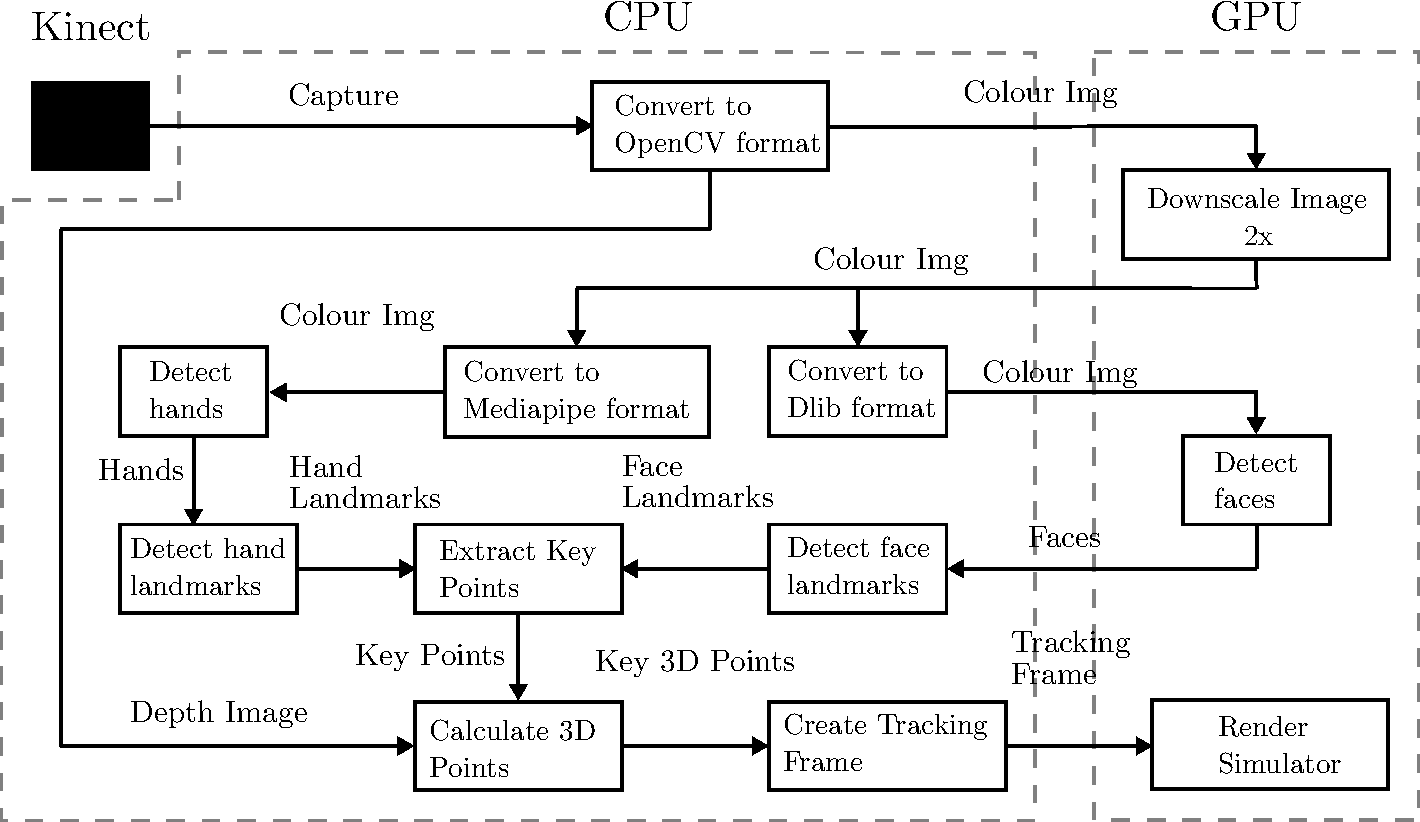
\includegraphics[width=1.0\linewidth]{./implementation/figures/tracking-system.pdf}
\end{figureBox}

%%%%%%%%%%%%%%%%%%%%%%%%%%%%%%%%%%%%%%%%%%%%%%%%%%%%%%%%%%%%%%%%%%%%%%%%%%%%%%%%%%%%%%%%%%%%

\subsection{Camera Positioning}

To ensure that the tracking system is calibrated correctly and that the user sees the correct perspective, it is crucial to know the relative position of the camera to the screen. Misalignment can lead to a distorted or incorrect user experience, where objects may appear to be in the wrong location or orientation relative to the user's point of view. To achieve this, the orientation of the camera and the dimensions of the screen must be accurately determined. We developed a calibration system to expedite the process of determining accurate position and orientation values. The calibration system operates as follows:

\begin{enumerate}[itemsep=-0.25em]
    \item The camera's position and orientation are measured in 3D space, and the screen's position is also measured in 3D space.
    \item The relative positions of the camera and screen are input into the system.
    \item The predicted position of the screen is rendered in 3D.
    \item The position of the screen is iteratively adjusted until the rendered position aligns with the actual position.
\end{enumerate}

An example of correct and incorrect calibration can be seen in Fig~\ref{fig:calibration}.

\begin{figureBox}[label={fig:calibration}, width=0.8\linewidth]{Display Calibration}
    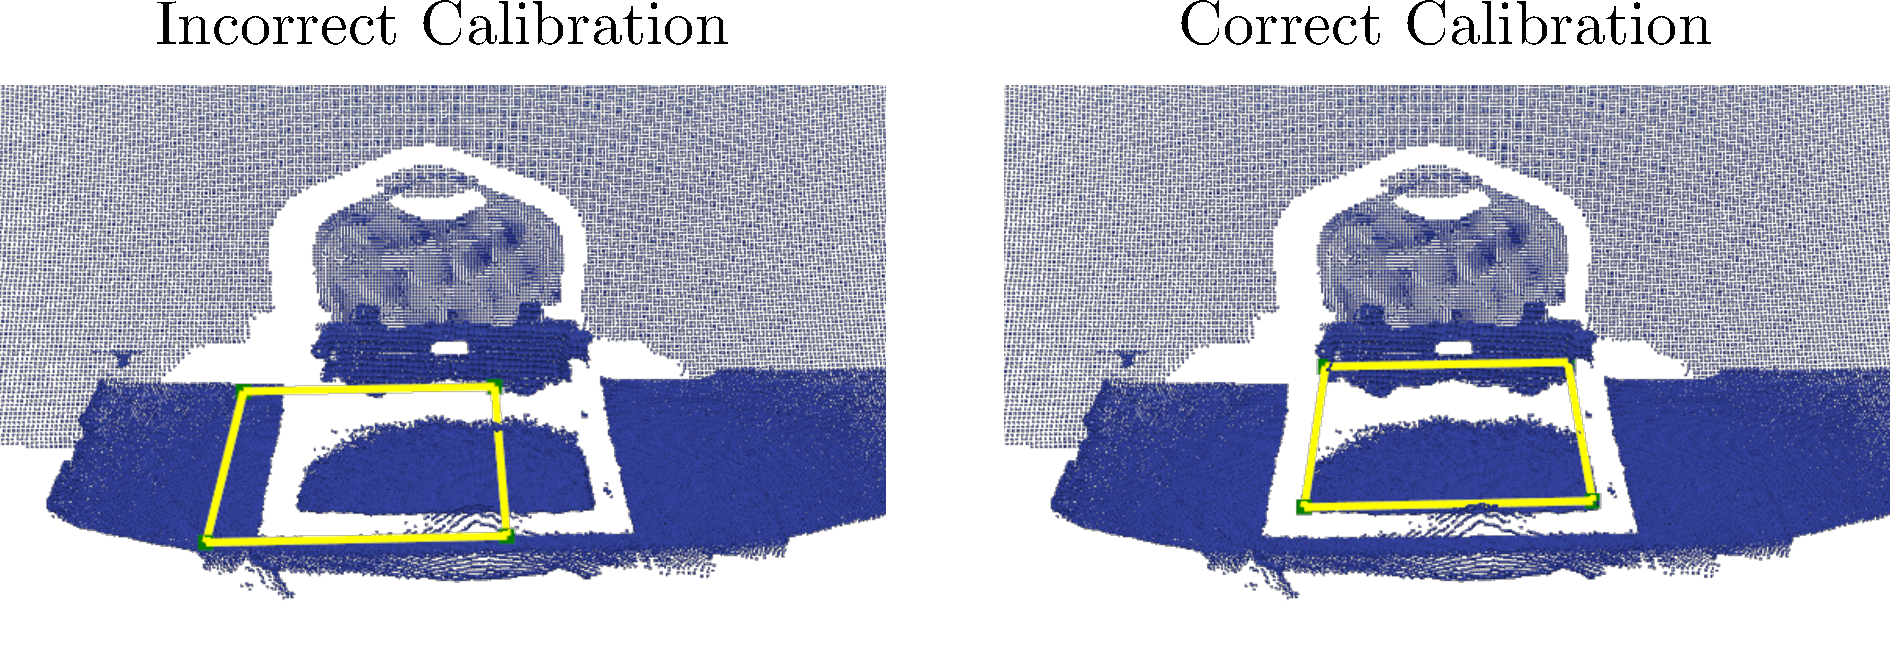
\includegraphics[width=1.0\linewidth]{./implementation/figures/calibration.pdf}
\end{figureBox}

